\section{Pruebas}
\label{sec:pruebas}

Las pruebas se dividen en dos grupos. El primero corresponde a la versión preliminar del firmware (filtros EMA y filtro de Kalman) y se conserva como antecedente, ya que motivó los cambios descriptos en la sección~\ref{sec:evolucion}. El segundo corresponde a las pruebas realizadas con la versión 2.3.0: la respuesta del sistema completo y la alimentación del receptor.

\subsection{Versión preliminar del firmware}
\label{sec:pruebas_preliminar}

Se analizó la utilidad de los filtros para cada medición realizada en el ESP32. Primero se observaron las mediciones del MPU6050 con el módulo totalmente quieto y luego con un pequeño movimiento. Para el \textit{pitch} resulta:

\begin{figure}[H]
 \centering
  \subfigure[\textit{Pitch} sin movimiento]{
    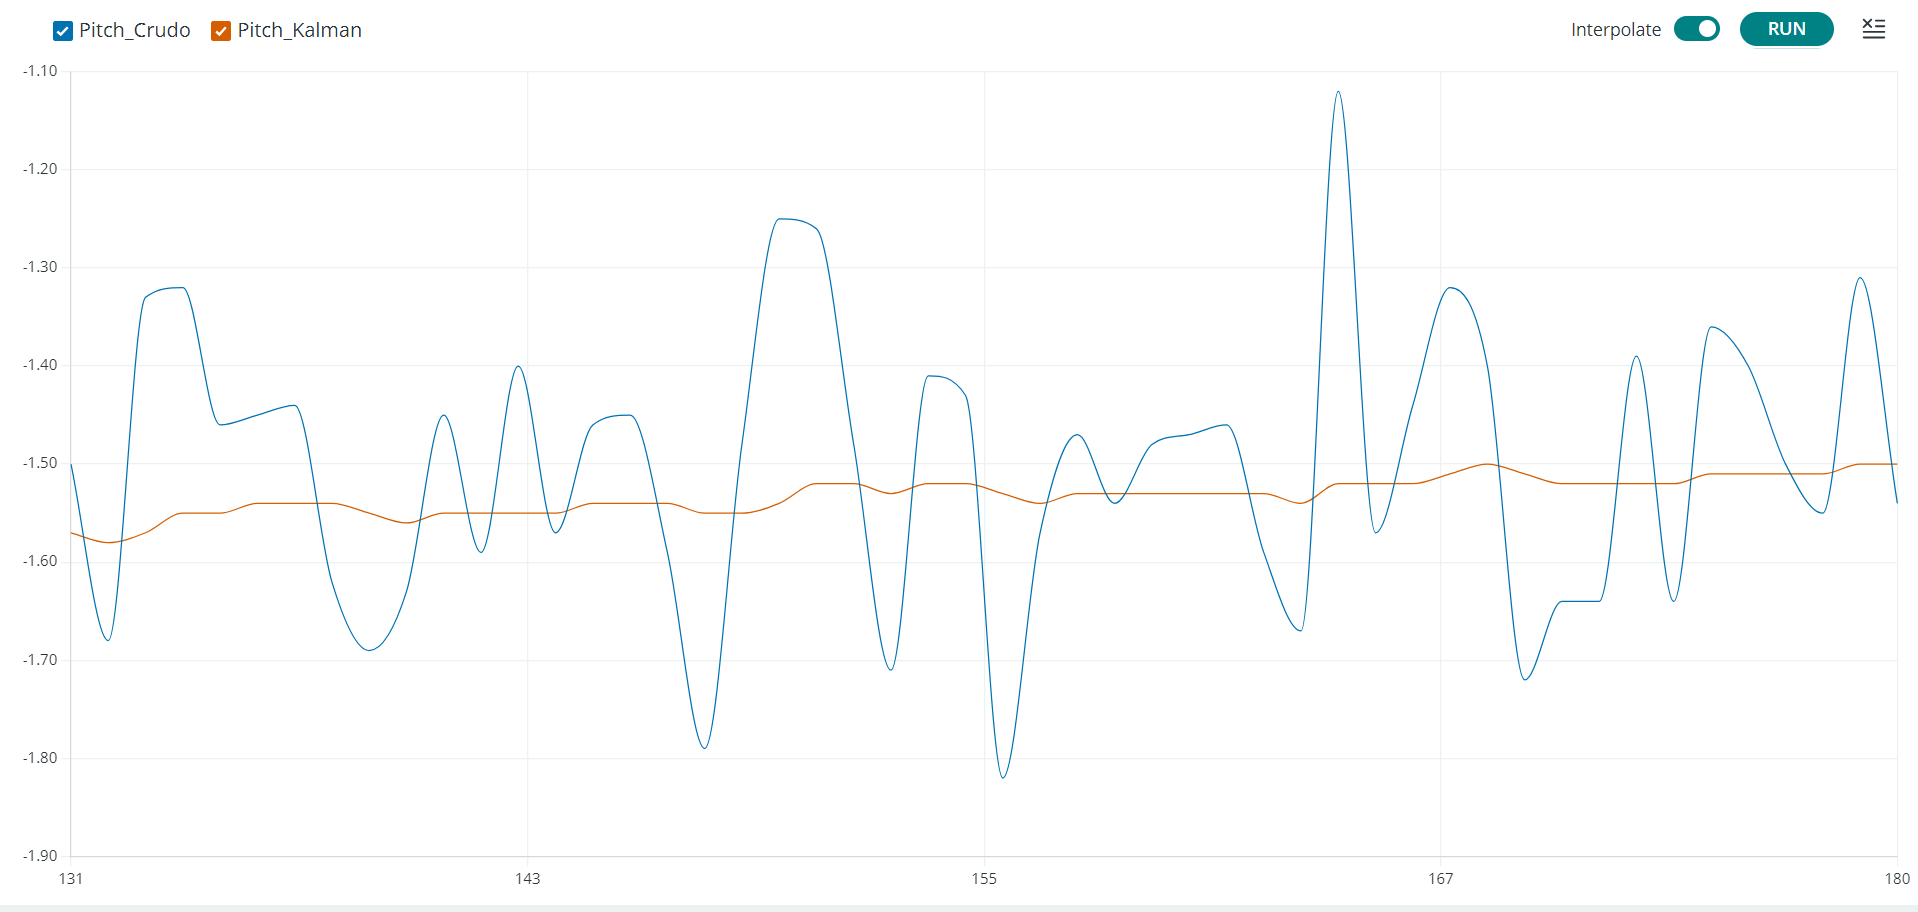
\includegraphics[width=0.45\textwidth]{Pitch_Ruido_Sin_Movimiento.png}}
  \subfigure[\textit{Pitch} con movimiento]{
    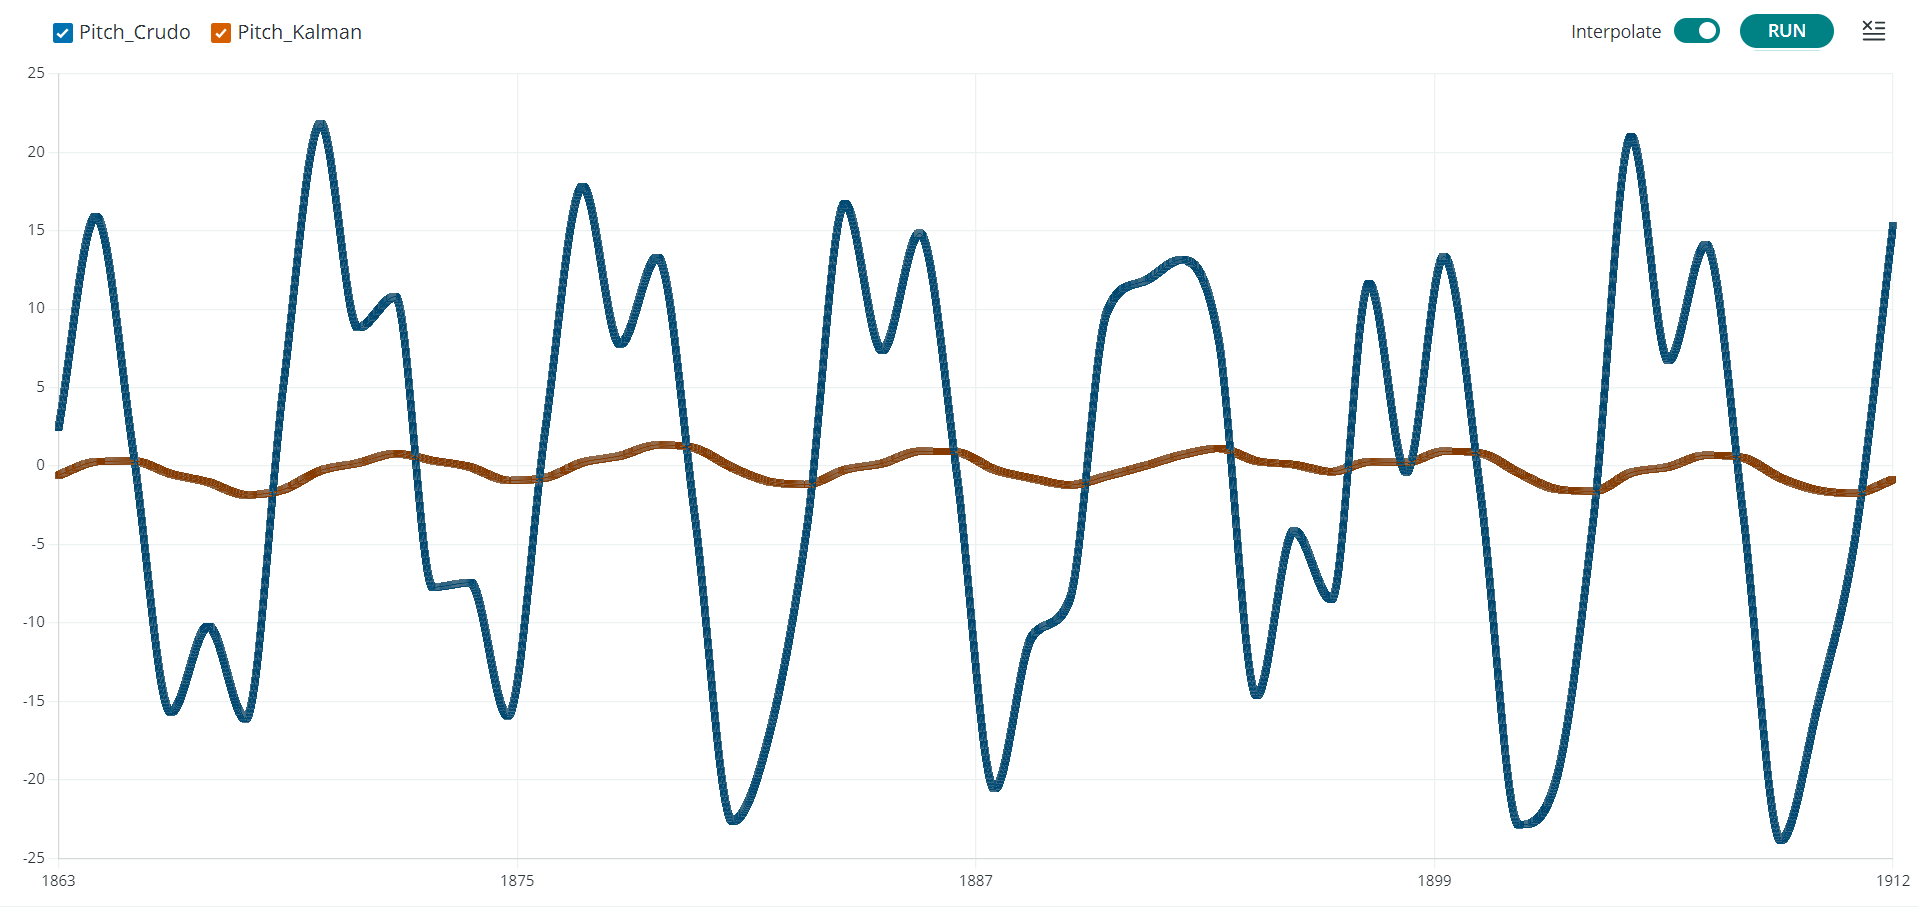
\includegraphics[width=0.45\textwidth]{Pitch_Ruido_Con_Movimiento.png}}
 \caption{Medición de \textit{pitch}.}
 \label{f:Ruido_Pitch}
\end{figure}

y para el \textit{roll} se observa:

\begin{figure}[H]
 \centering
  \subfigure[\textit{Roll} sin movimiento]{
    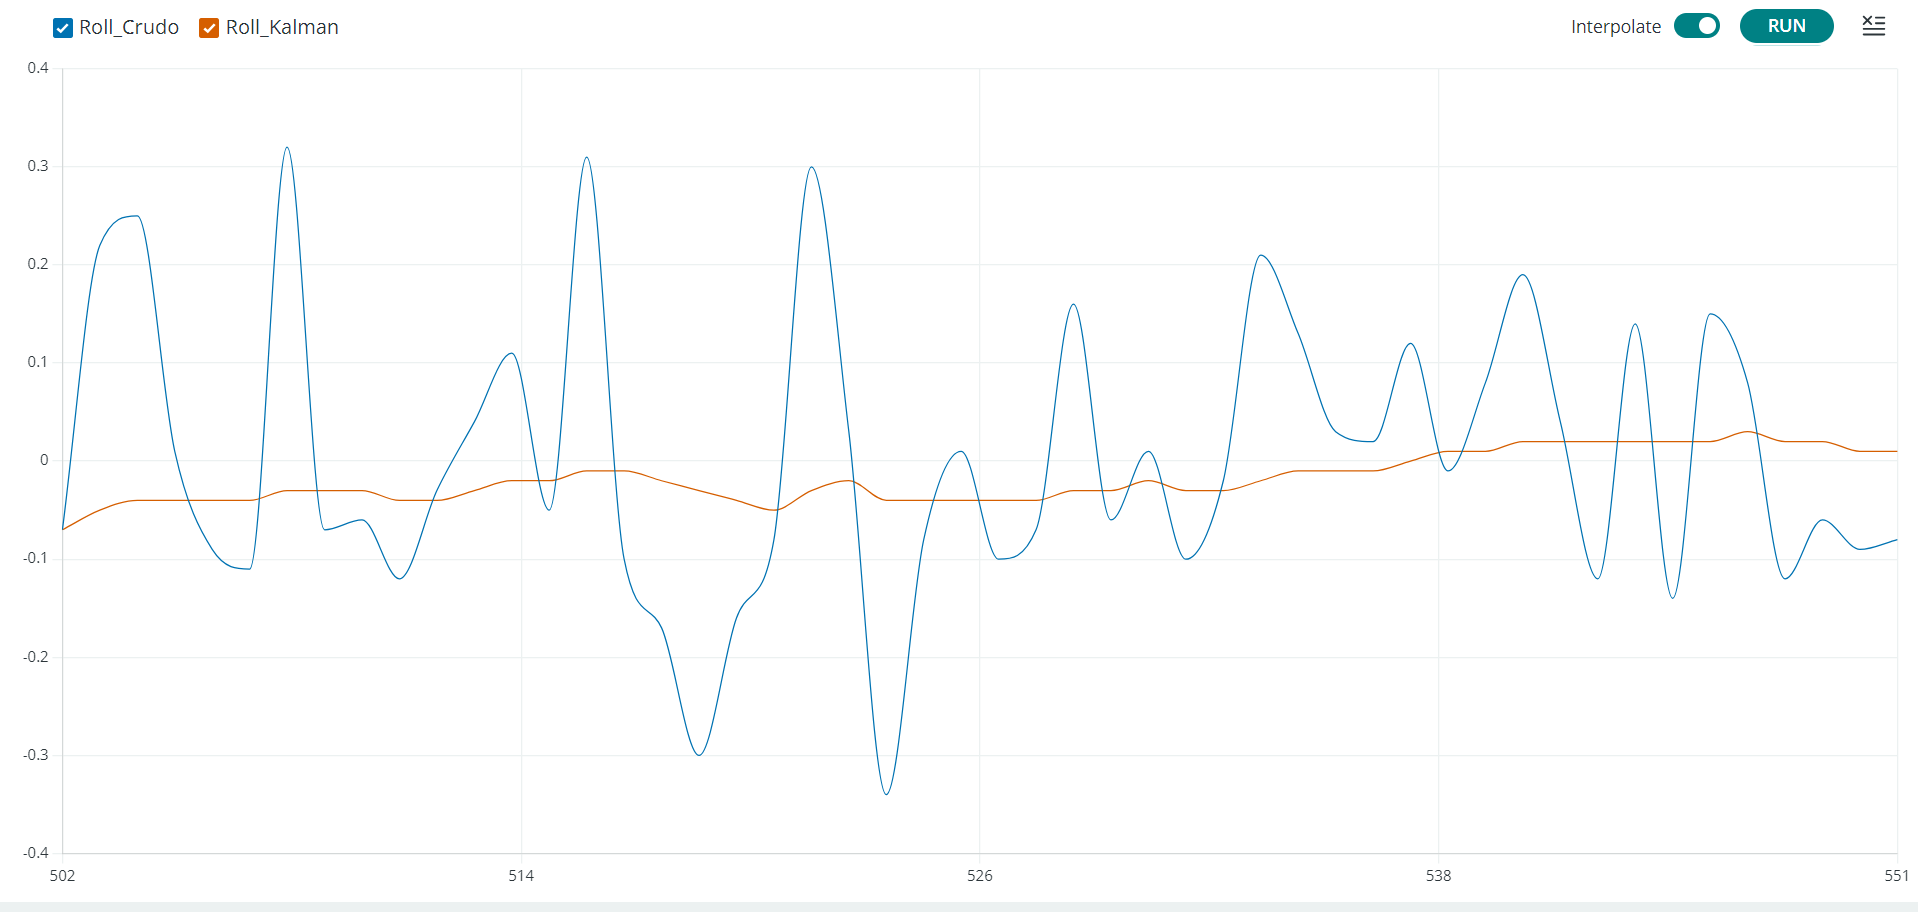
\includegraphics[width=0.45\textwidth]{Roll_Ruido_Sin_Movimiento.png}}
  \subfigure[\textit{Roll} con movimiento]{
    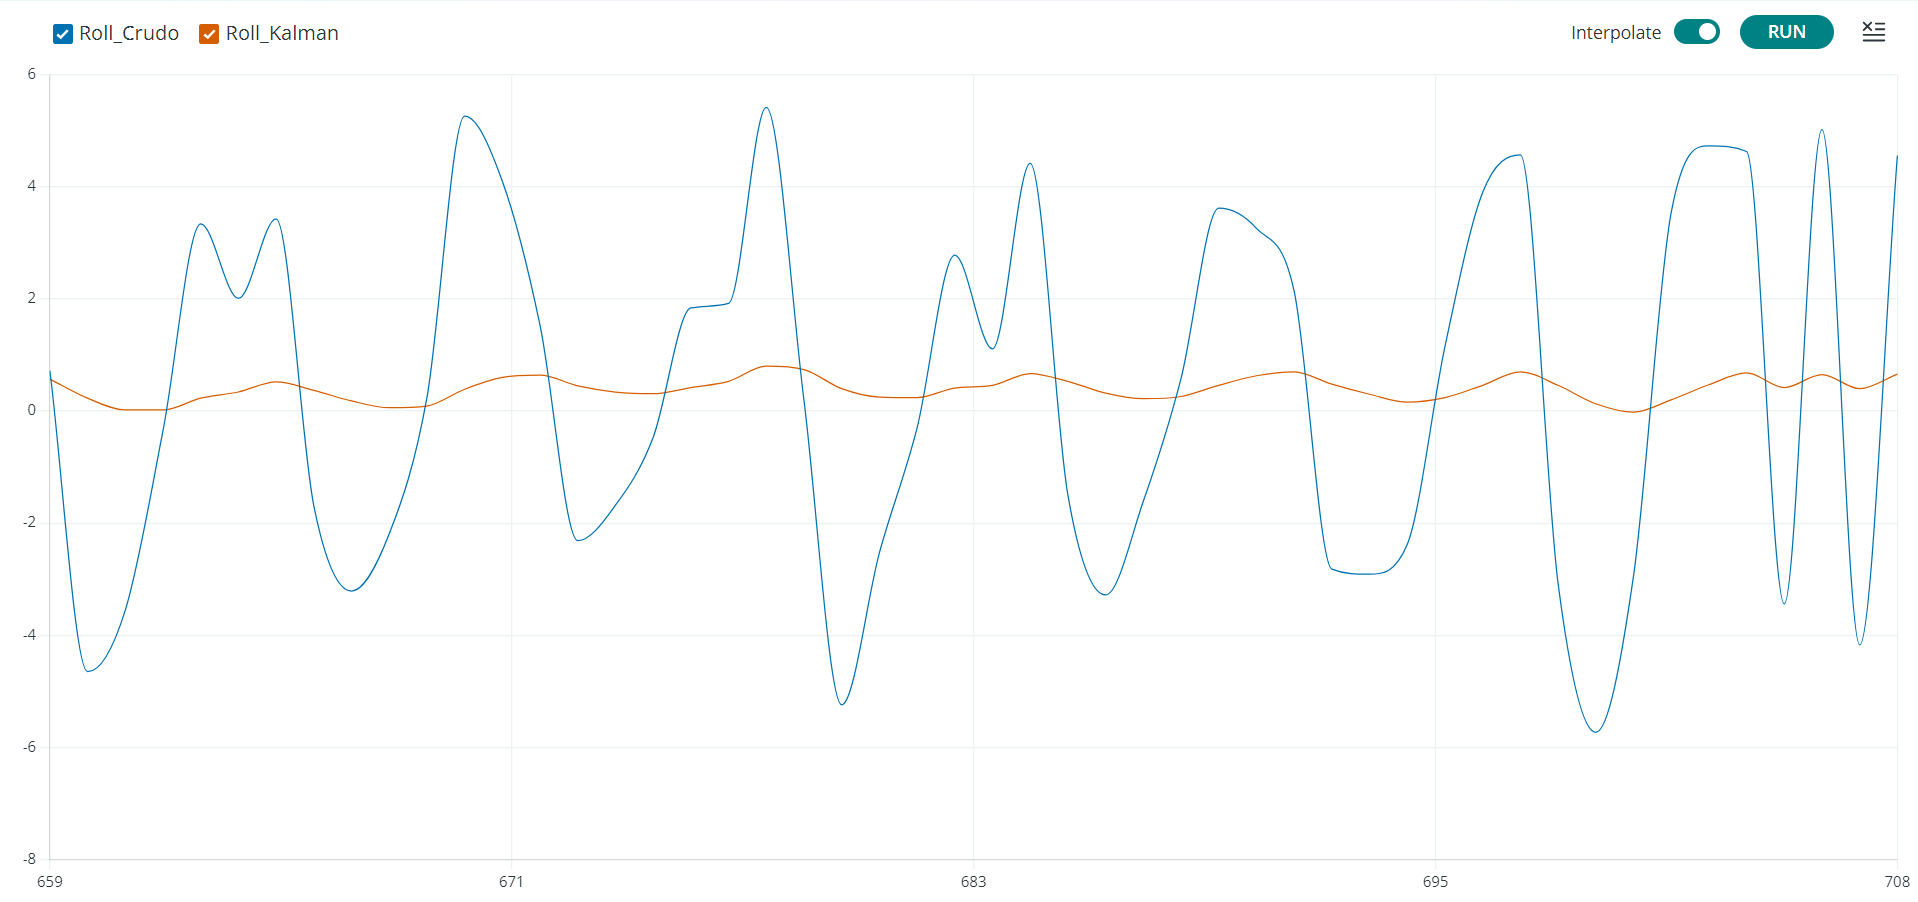
\includegraphics[width=0.45\textwidth]{Roll_Ruido_Con_Movimiento.png}}
 \caption{Medición de \textit{roll}.}
 \label{f:Ruido_Roll}
\end{figure}

Luego se analizó el comportamiento de los potenciómetros, comparando los datos leídos en crudo con los filtrados:

\begin{figure}[H]
 \centering
  \subfigure[Cambio lento]{
    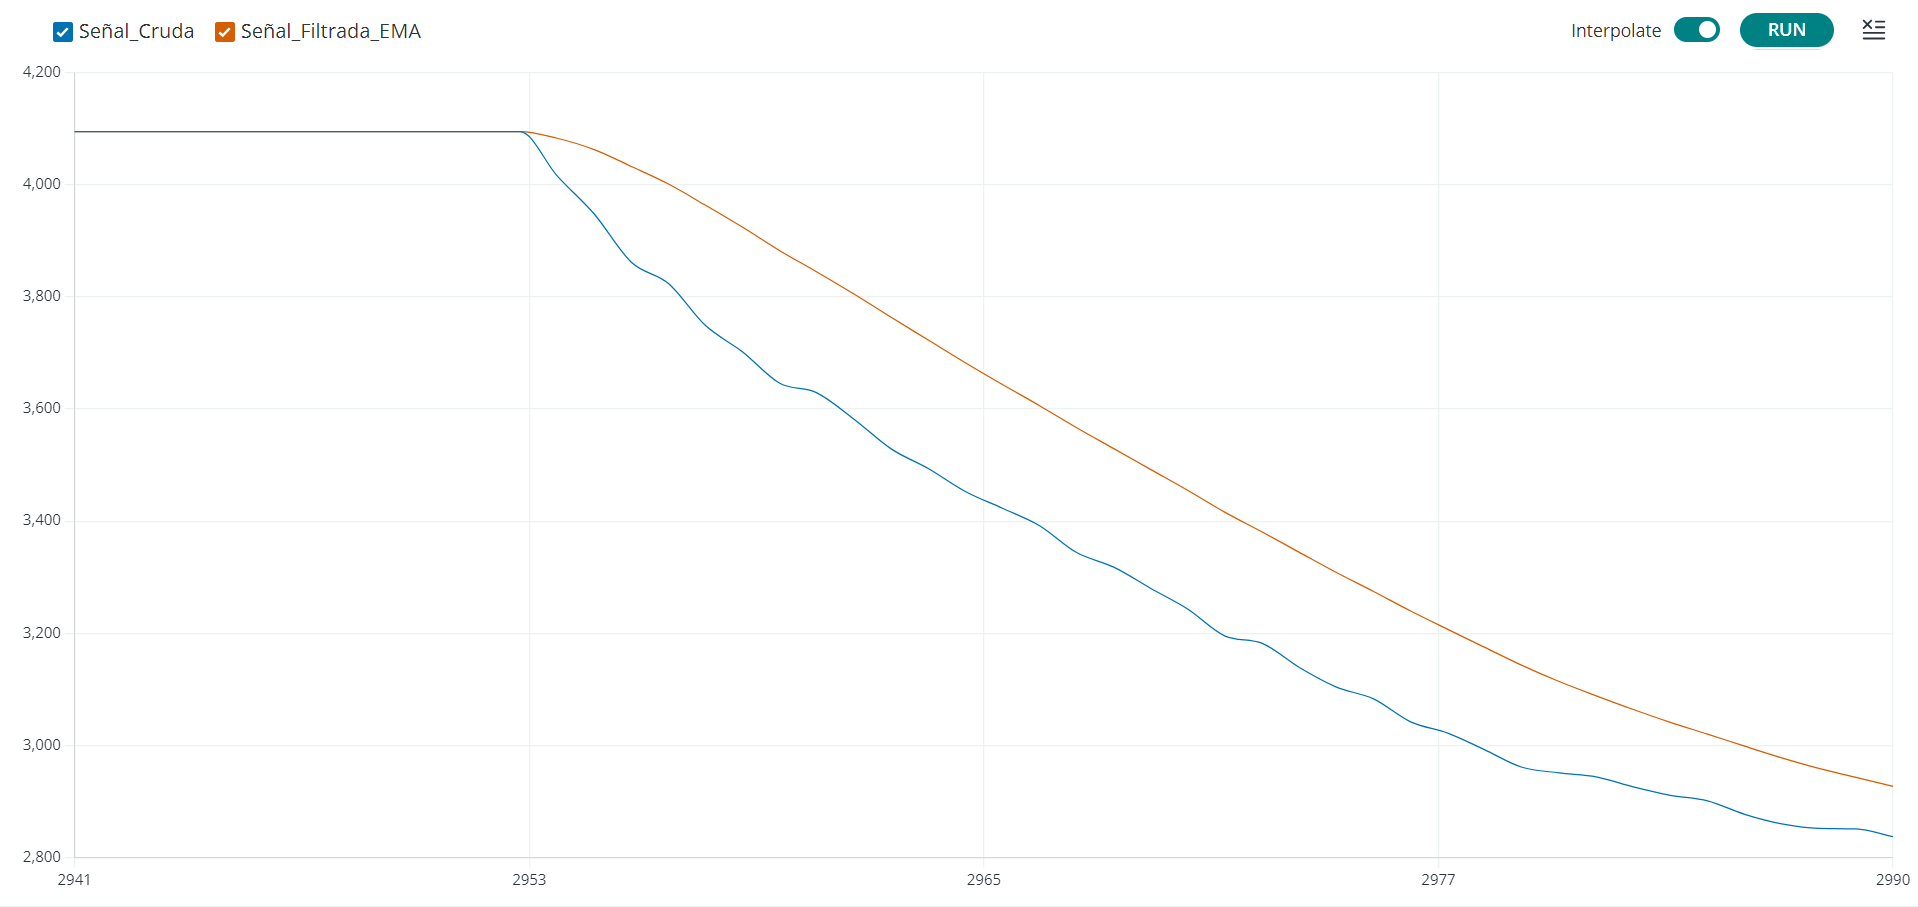
\includegraphics[width=0.45\textwidth]{Pote_Ruido.png}}
  \subfigure[Cambio brusco]{
    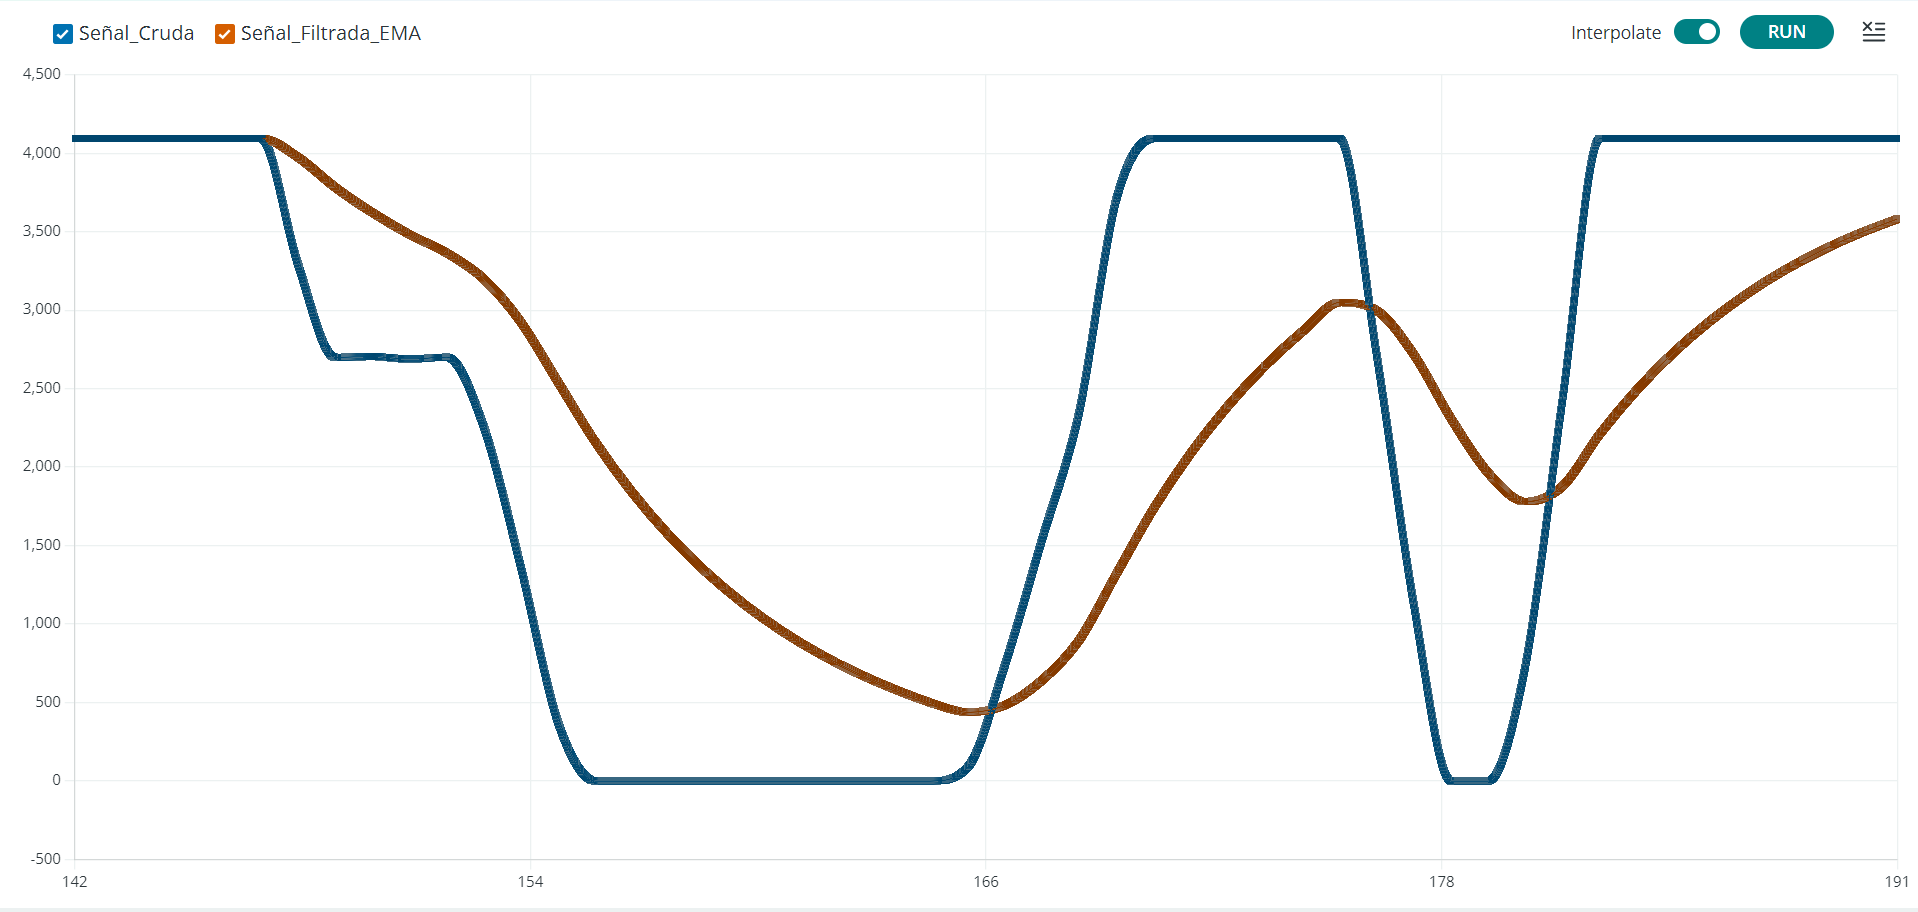
\includegraphics[width=0.45\textwidth]{Pote_Ruido_1.png}}
 \caption{Respuesta de un potenciómetro.}
 \label{f:Ruido_Potenciometros}
\end{figure}

Con el filtrado, la respuesta de la lectura es más lenta. En la versión preliminar esto se consideró deseable para proteger el mecanismo; sin embargo, sumado al filtro del receptor, el retardo resultó perceptible, lo que motivó los cambios descriptos en la sección~\ref{sec:evolucion}.

A continuación se observa la respuesta del sistema completo, transmisor y receptor:

\begin{figure}[H]
 \centering
  \subfigure[Desplazamiento vertical]{
    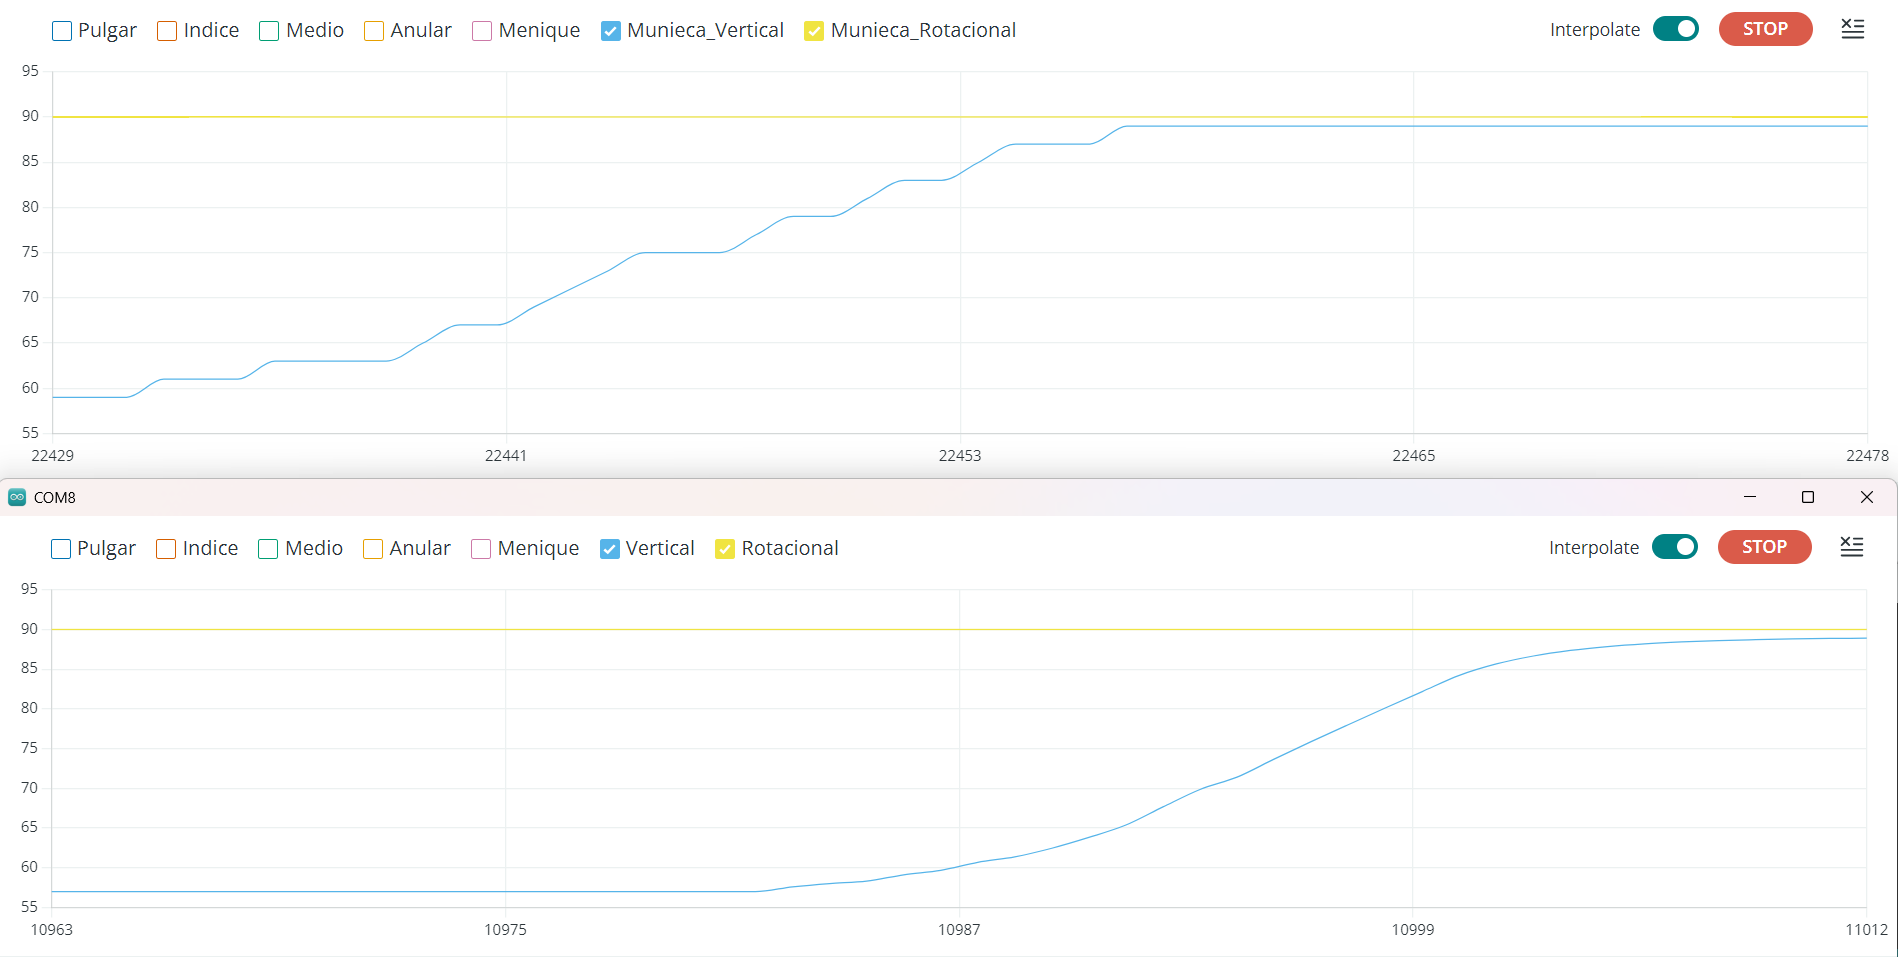
\includegraphics[width=0.47\textwidth]{Transmicion_1.png}}
  \subfigure[Rotación]{
    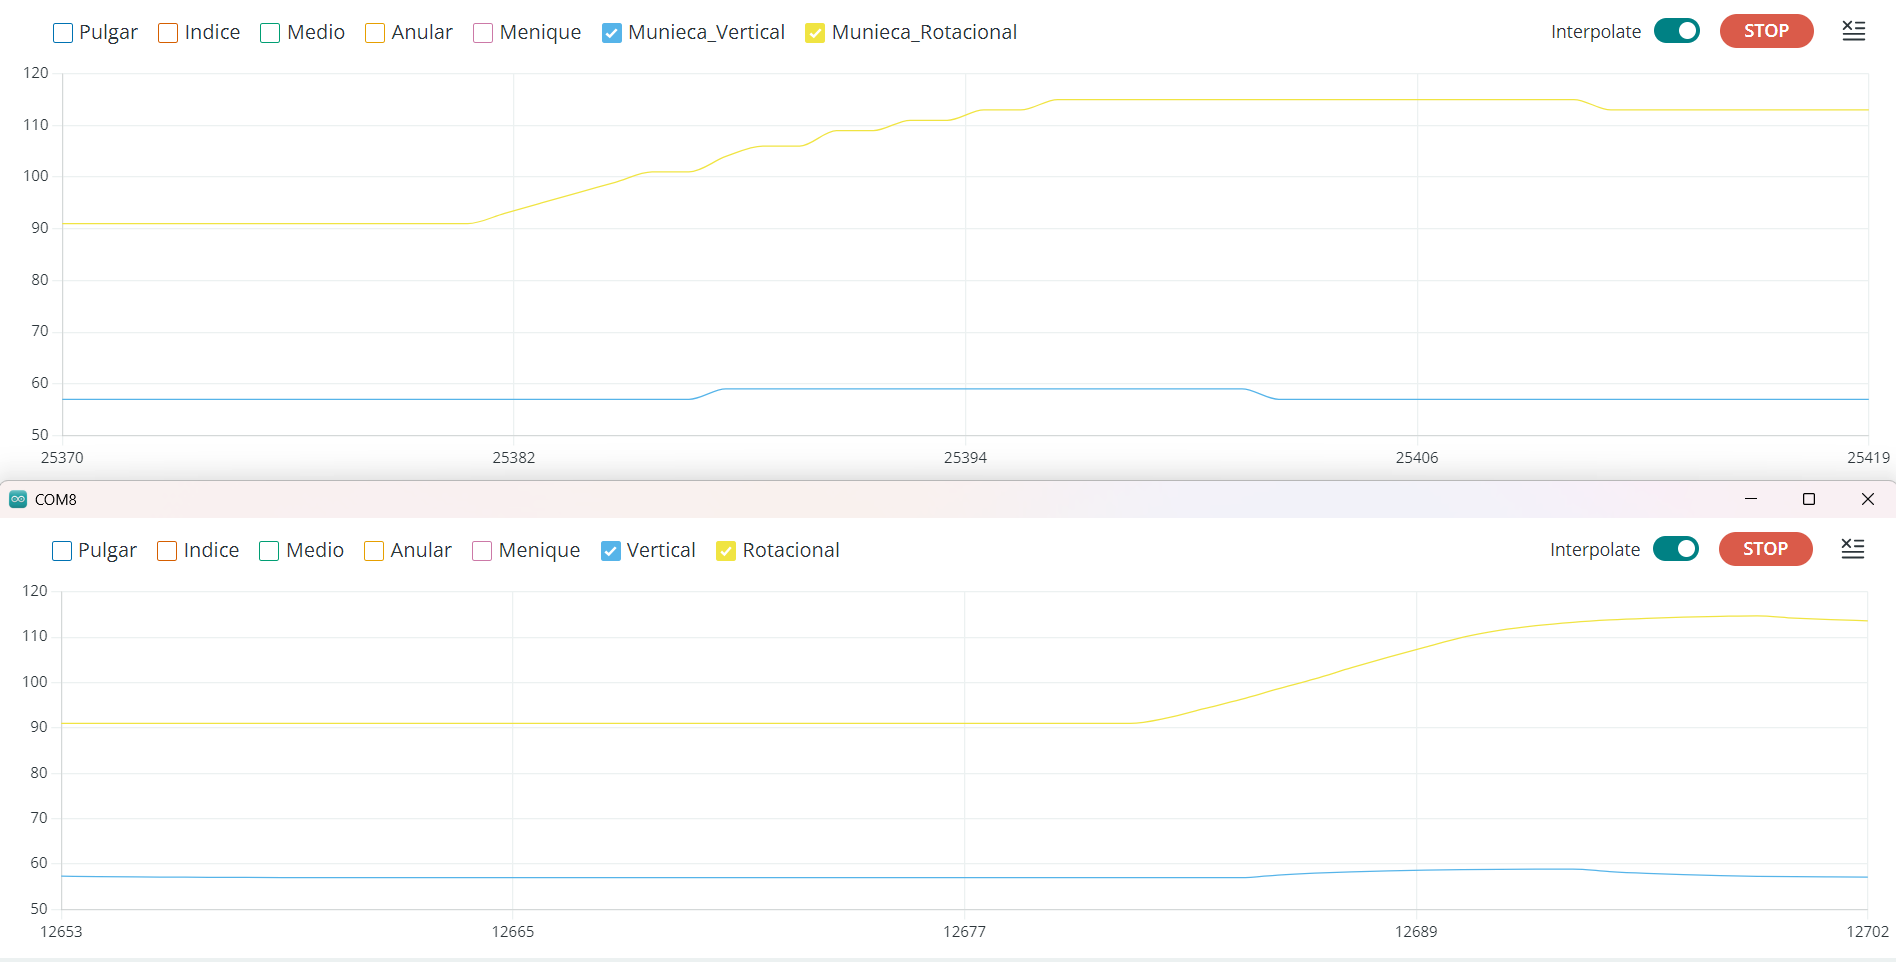
\includegraphics[width=0.47\textwidth]{Transmicion_2.png}}
  \subfigure[Subir dedo]{
    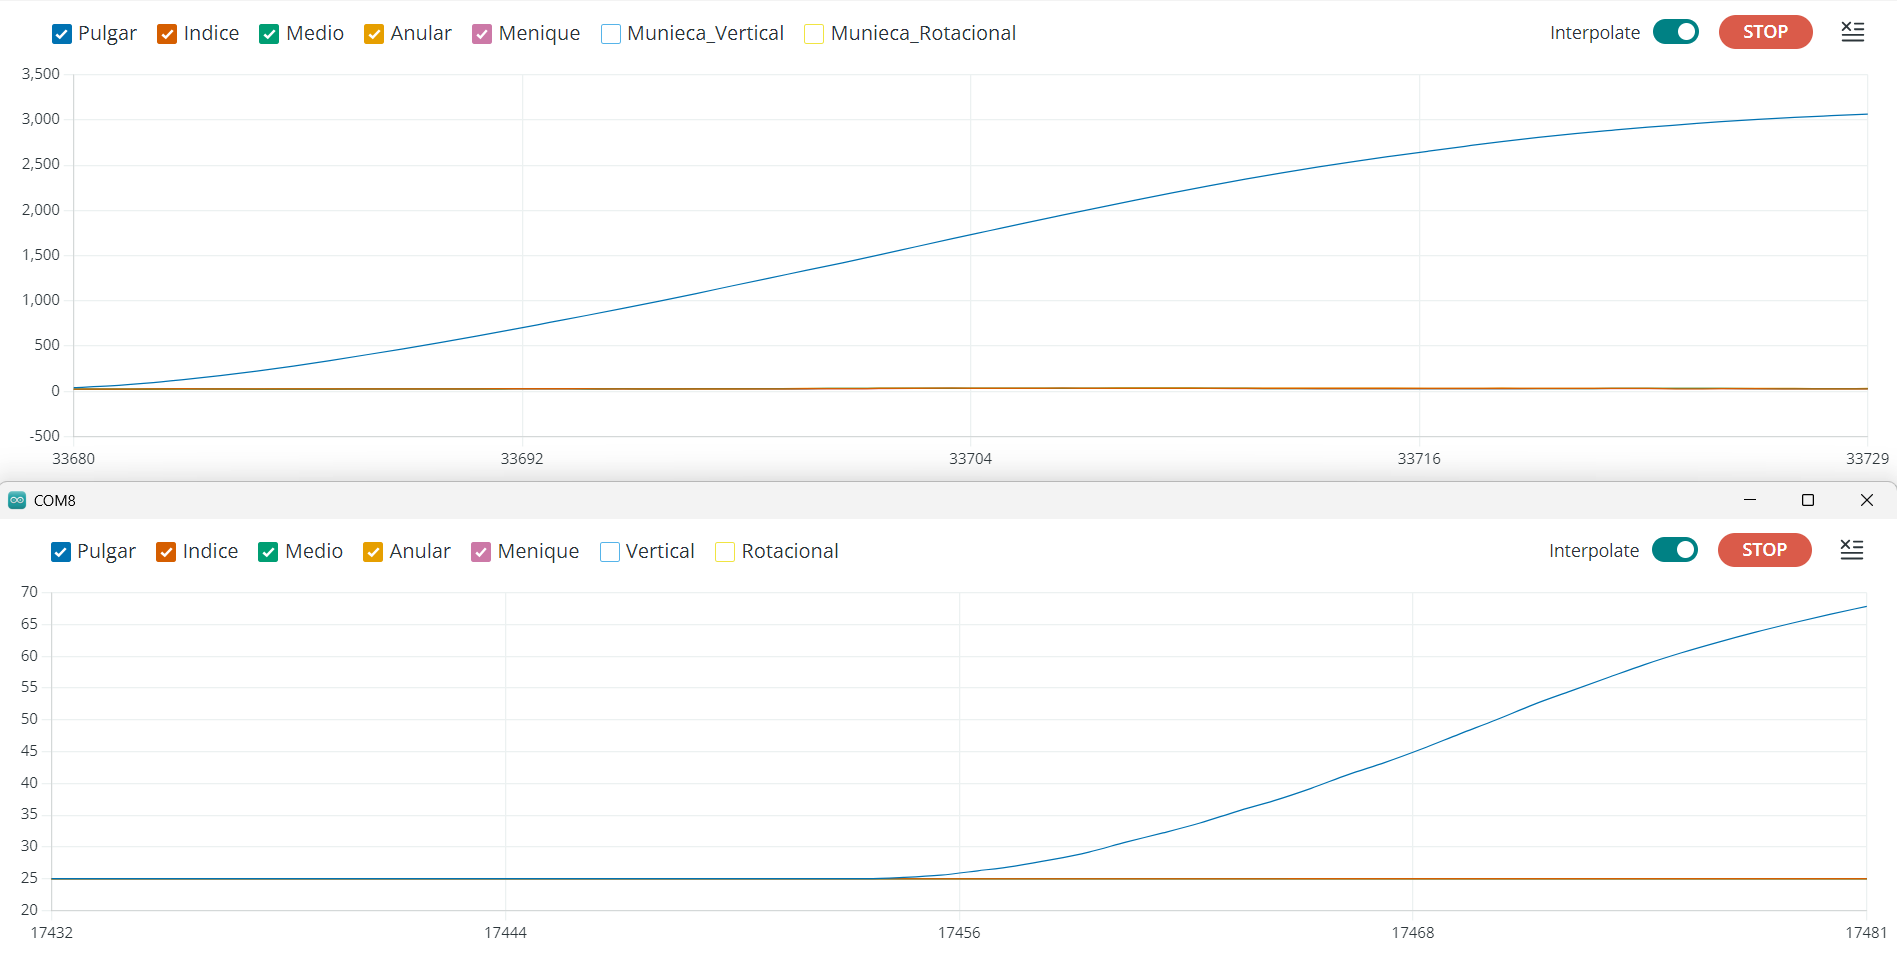
\includegraphics[width=0.47\textwidth]{Transmicion_3.png}}
  \subfigure[Bajar dedo]{
    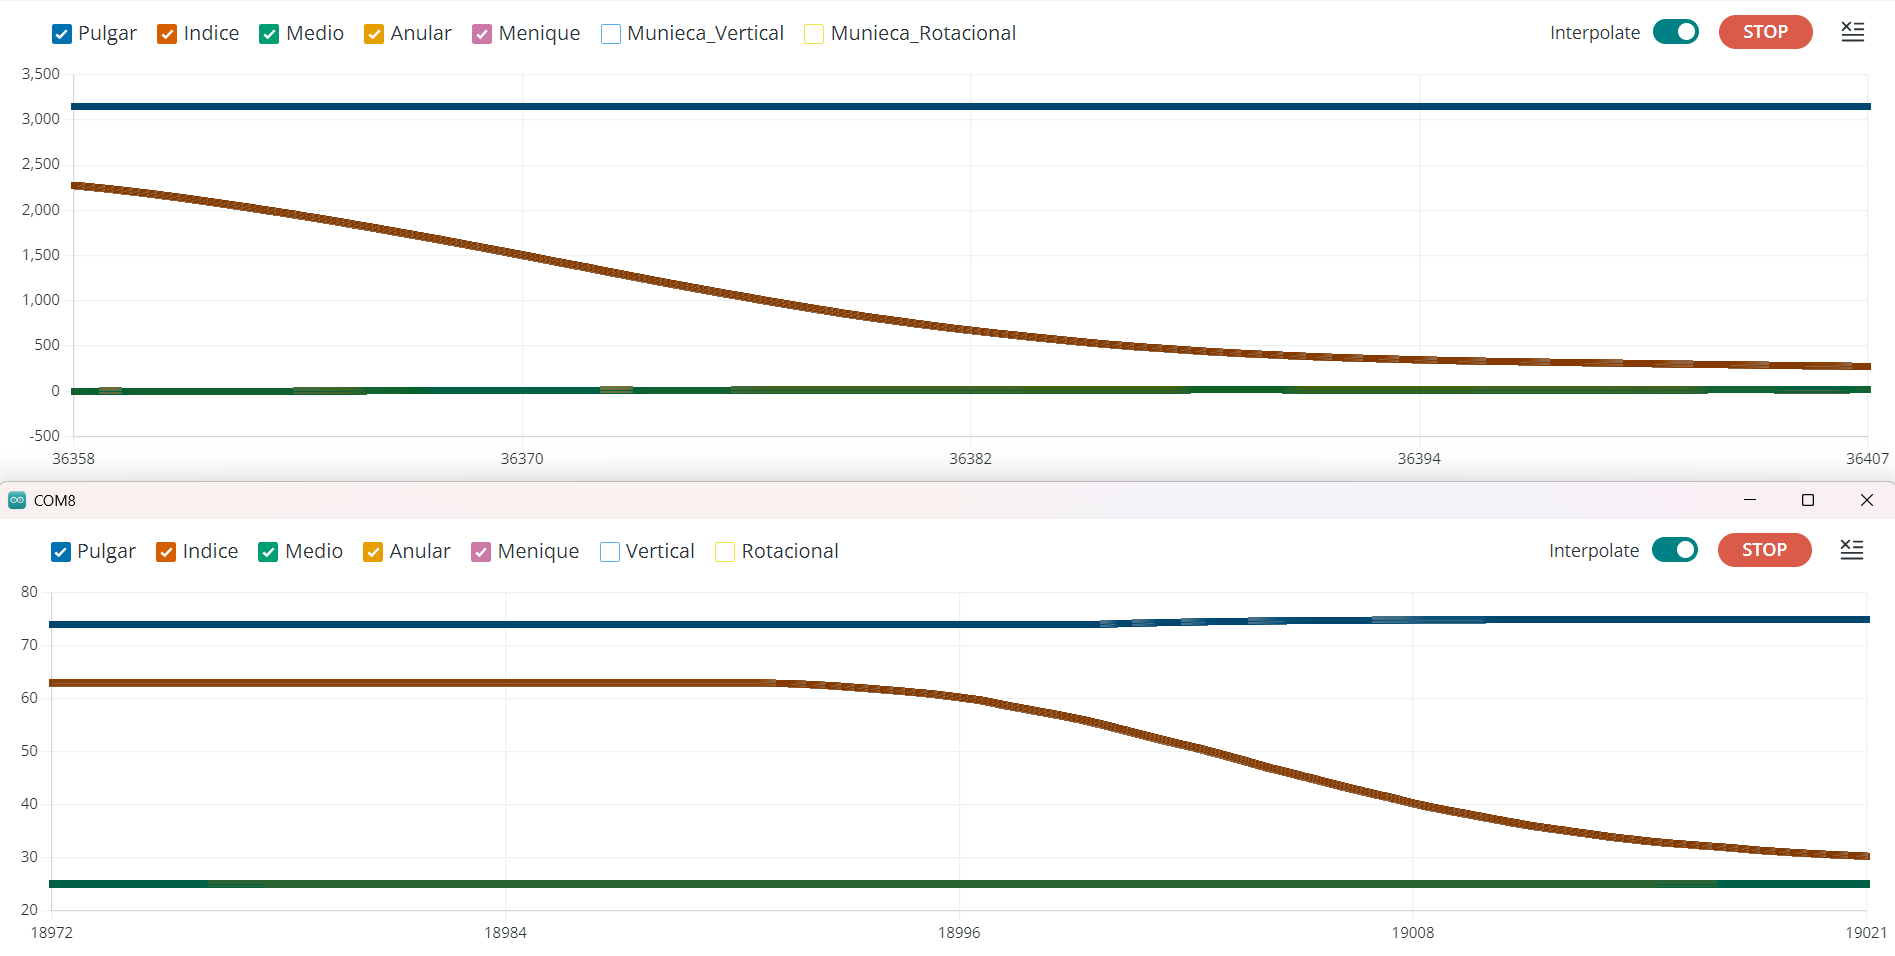
\includegraphics[width=0.47\textwidth]{Transmicion_4.png}}
 \caption{Respuesta del sistema.}
 \label{f:Respuesta_Sistema}
\end{figure}

Se observa un pequeño retardo entre la lectura en el transmisor y la réplica en el receptor. Estas curvas no permiten cuantificarlo: la telemetría se enviaba a \SI{5}{\hertz} por USB, con una resolución de \SI{200}{\milli\second}, y la hora de cada muestra la asignaba la computadora. La estimación del retardo se presenta en la sección~\ref{sec:latencia}.

\subsection{Respuesta del sistema (versión 2.3.0)}
\label{sec:pruebas_respuesta}

Para comparar la orden del guante con la posición que aplica la mano se compiló el firmware 2.3.0 de ambos nodos con una telemetría opcional en formato CSV a \SI{50}{\hertz}. En cada paquete, el transmisor imprime por USB su número de secuencia y los siete ángulos enviados; el receptor imprime el número de secuencia del paquete procesado y los siete ángulos que escribió en los servos, junto con su propio \texttt{millis()}. Un programa en MATLAB lee los dos puertos serie a la vez y, cuando llega una línea del receptor, busca la línea del transmisor con el mismo número de secuencia y la ubica en el instante del reloj del receptor en que ese paquete fue procesado. De este modo ambas curvas quedan en la misma base de tiempo sin depender de la hora en que la computadora recibe cada línea.

Por esa misma razón, el corrimiento entre las curvas no representa la latencia del enlace inalámbrico (que no se mide con este método, ya que ambas curvas se ubican al procesar el paquete en el receptor), sino el efecto del limitador de velocidad y de la banda muerta del receptor (sección~\ref{sec:slew}). Las figuras~\ref{fig:respuesta_dedos} y~\ref{fig:respuesta_muneca} muestran, para cada señal, la orden del transmisor (arriba) y la posición aplicada por el receptor (abajo). El eje de tiempo de las capturas está en milisegundos del receptor multiplicados por $10^5$ (el factor de escala que agrega MATLAB quedó fuera de las capturas): cada división corresponde a \SI{500}{\milli\second} y la ventana completa a unos \SI{5}{\second}.

\begin{figure}[H]
 \centering
  \subfigure[Pulgar]{
    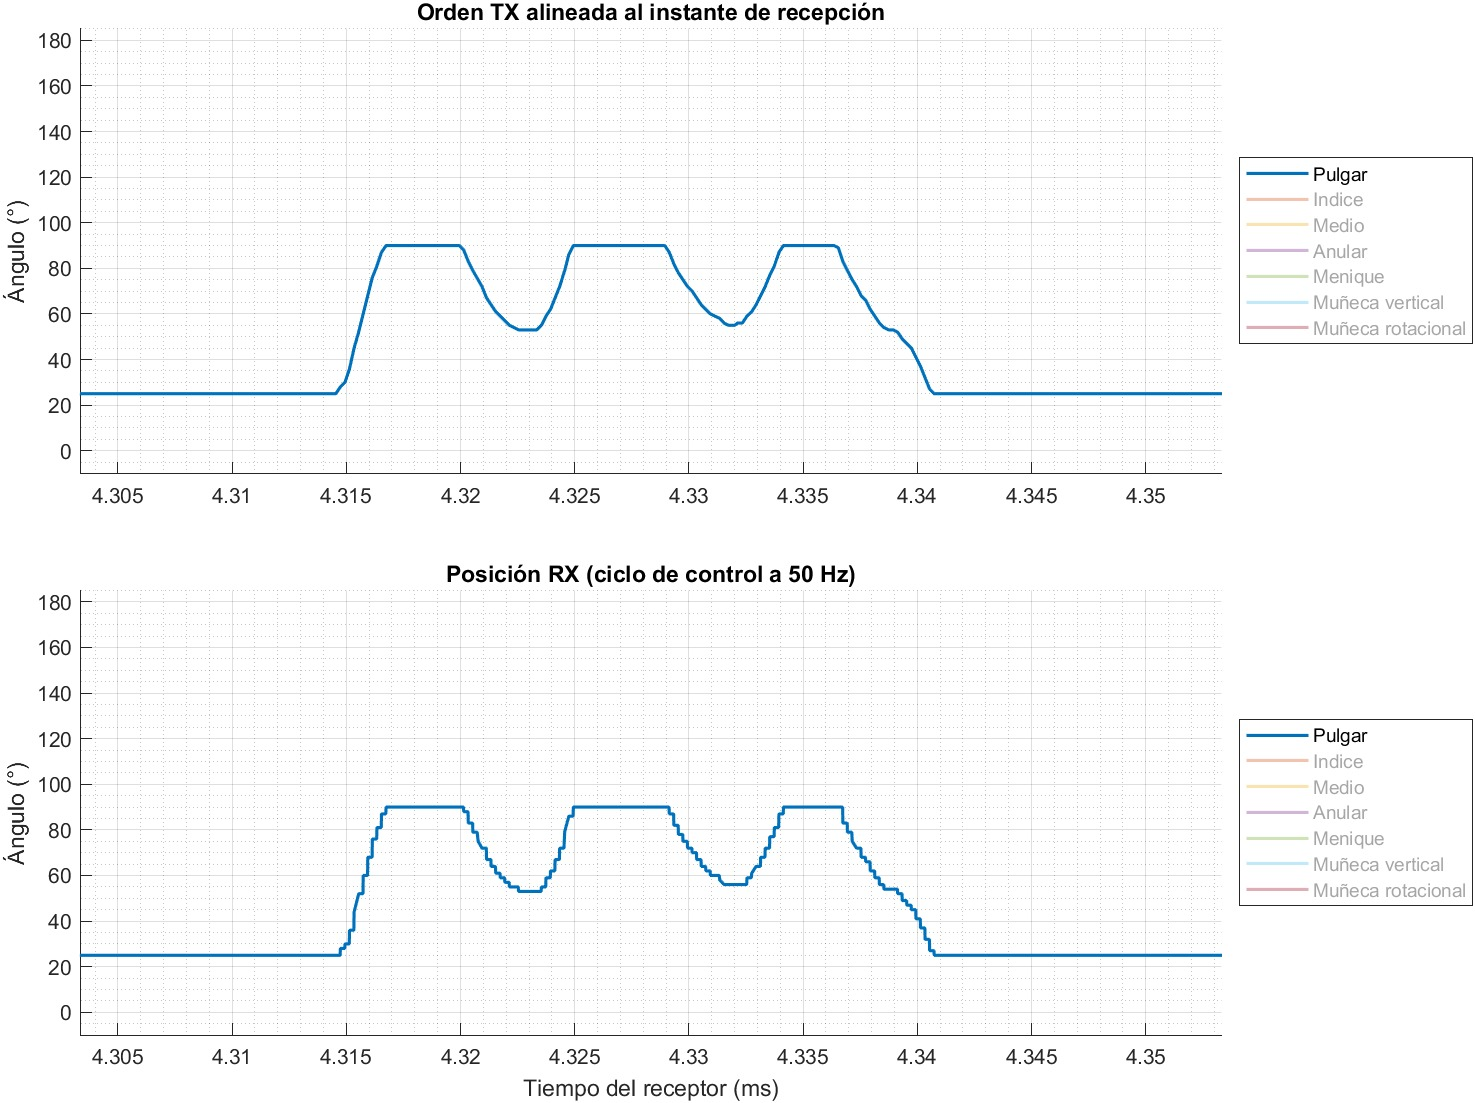
\includegraphics[width=0.48\textwidth]{Mediciones/P16_matlab_pulgar.jpg}}
  \subfigure[Índice]{
    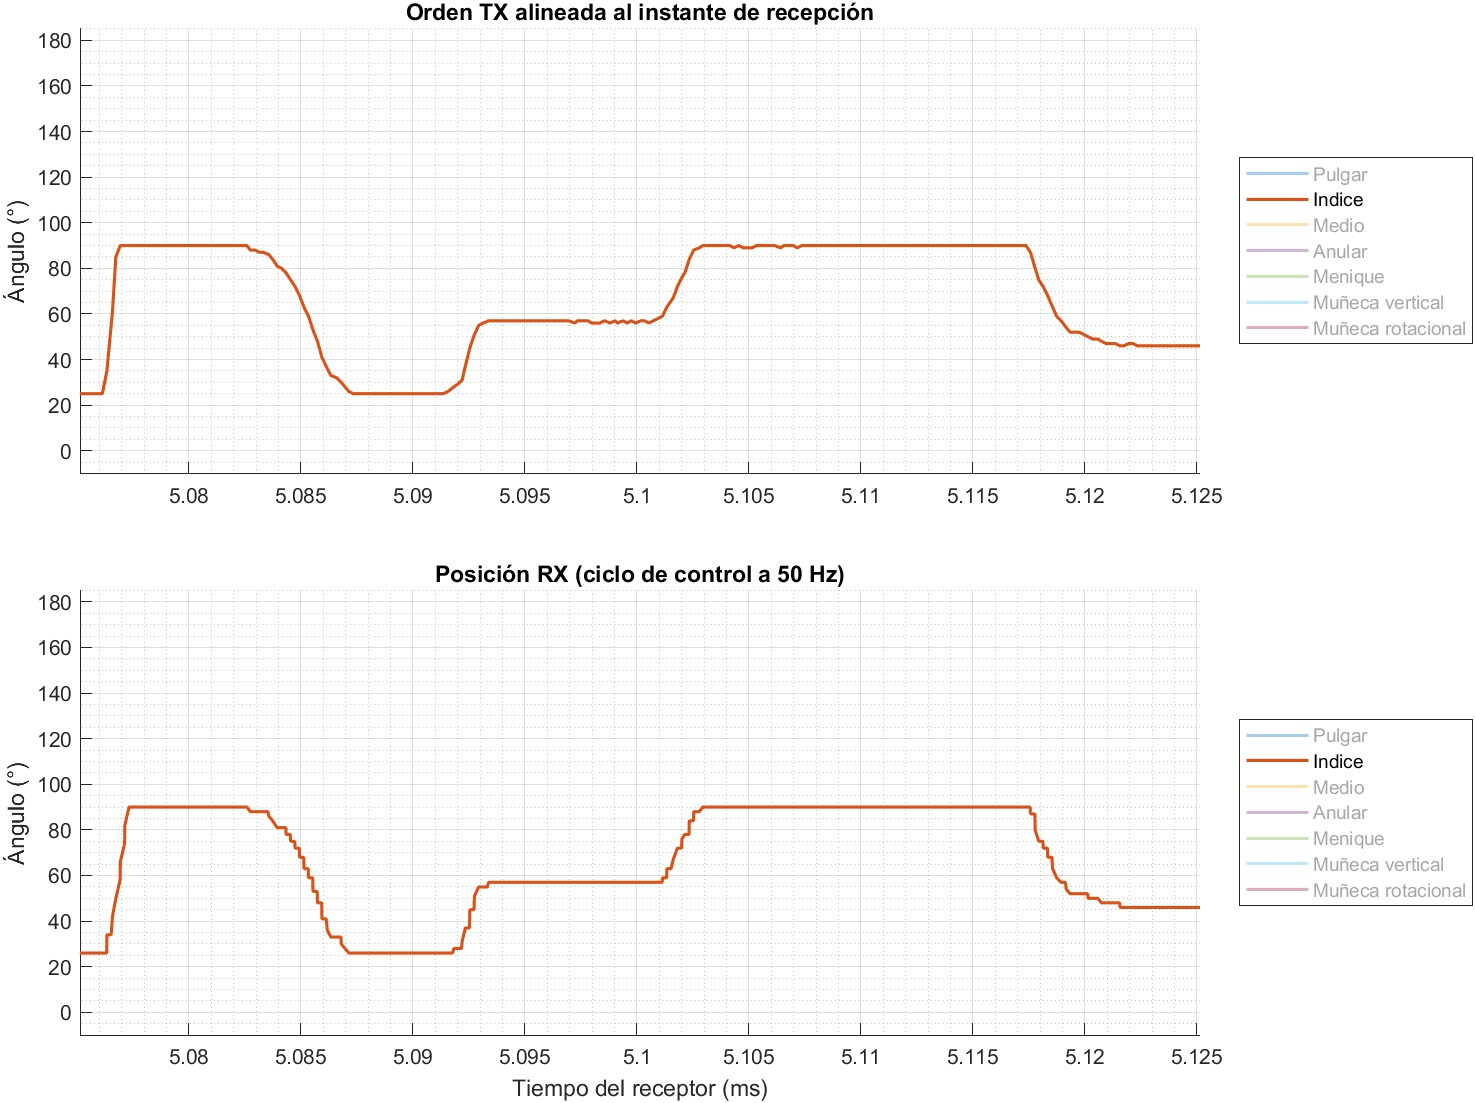
\includegraphics[width=0.48\textwidth]{Mediciones/P16_matlab_indice.jpg}}
 \caption{Respuesta de los dedos: orden del transmisor alineada por número de secuencia (arriba) y posición aplicada por el receptor (abajo).}
 \label{fig:respuesta_dedos}
\end{figure}

\begin{figure}[H]
 \centering
  \subfigure[Muñeca rotacional]{
    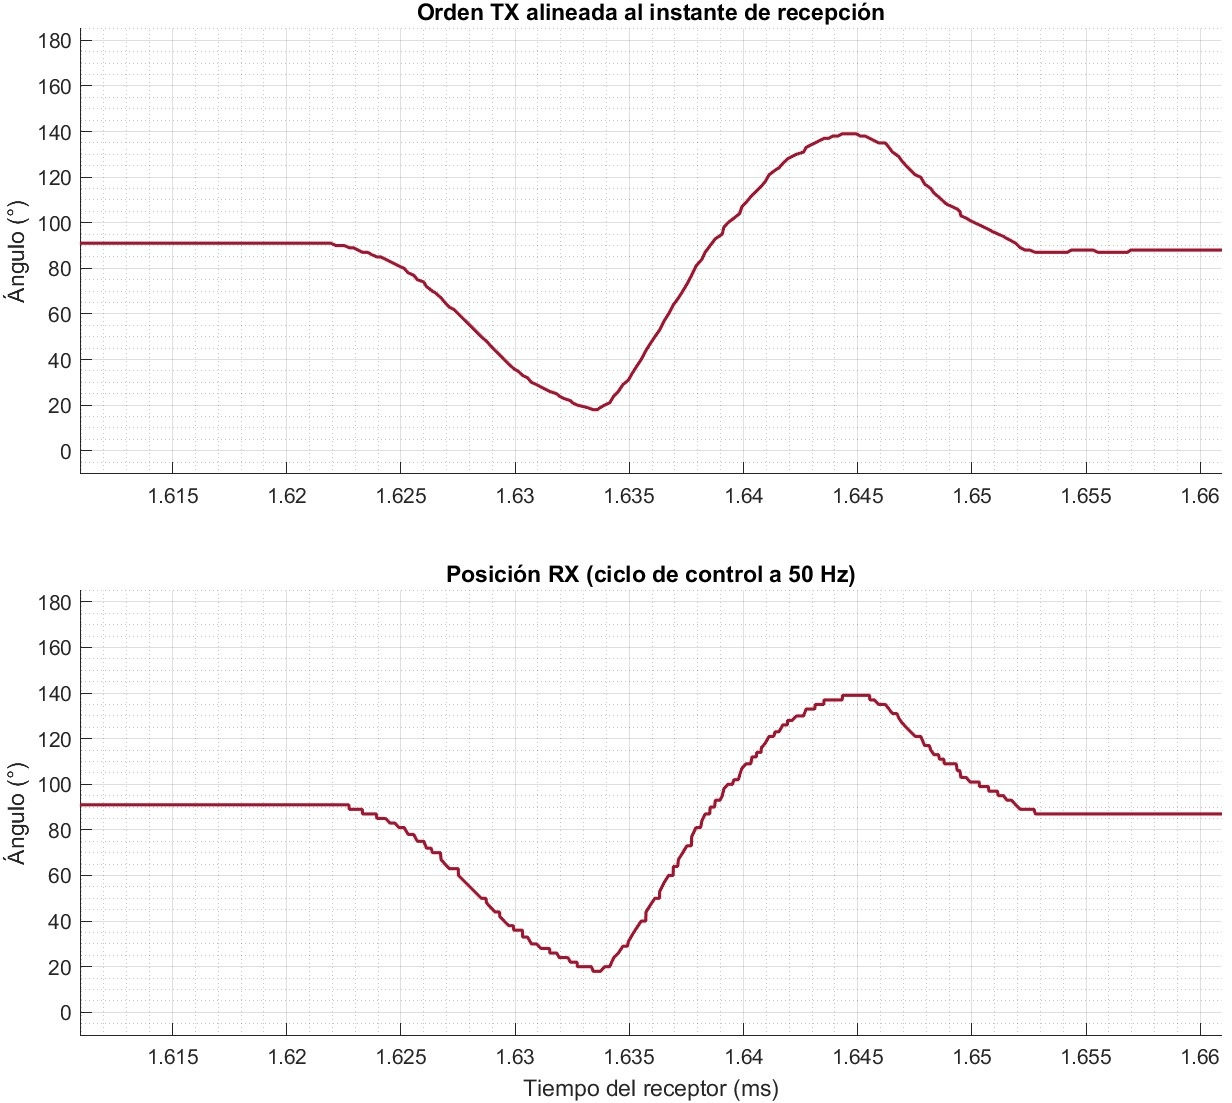
\includegraphics[width=0.48\textwidth]{Mediciones/P16_matlab_muneca_rotacional.jpg}}
  \subfigure[Muñeca vertical]{
    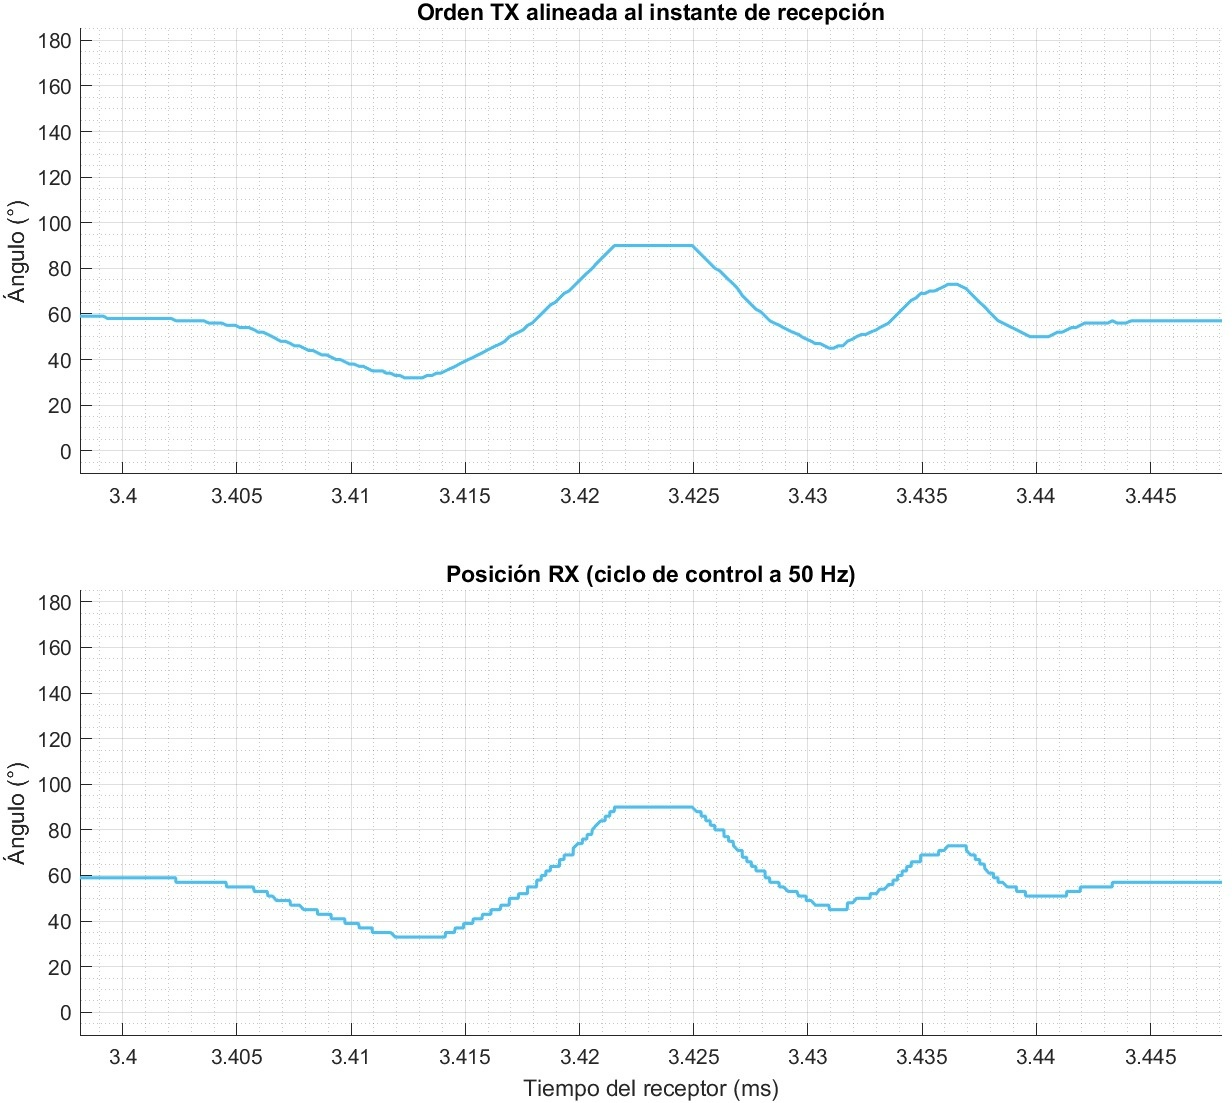
\includegraphics[width=0.48\textwidth]{Mediciones/P16_matlab_muneca_vertical.jpg}}
 \caption{Respuesta de la muñeca: orden del transmisor alineada por número de secuencia (arriba) y posición aplicada por el receptor (abajo).}
 \label{fig:respuesta_muneca}
\end{figure}

De las capturas se observa lo siguiente:

\begin{itemize}
    \item \textbf{Seguimiento.} En las cuatro señales la posición del receptor reproduce la forma de la orden, tanto en los movimientos completos (el pulgar entre \SI{25}{\degree} y \SI{90}{\degree}, la rotación de la muñeca entre \SI{18}{\degree} y \SI{139}{\degree}) como en las posiciones intermedias (el índice detenido en unos \SI{57}{\degree} y \SI{46}{\degree}). A la escala de las capturas no se distingue un retraso entre ambas curvas.
    \item \textbf{Saturación en los límites.} Las órdenes de los dedos se recortan en \SIrange{25}{90}{\degree} y la de la muñeca vertical en \SI{90}{\degree}, y el receptor se mantiene dentro de esos rangos.
    \item \textbf{Escalonamiento.} La posición del receptor se grafica en escalones, uno por ciclo de control: en cada paquete el servo recibe una nueva posición, que el limitador de velocidad acota a \SI{8}{\degree} por ciclo en los dedos y a \SIrange{4}{5}{\degree} en la muñeca. En los movimientos registrados los pasos de la orden son, en general, menores que esos límites, por lo que el receptor la sigue paquete a paquete.
    \item \textbf{Banda muerta.} Las pequeñas variaciones de \SI{1}{\degree} de la orden durante las mesetas (por ejemplo, el índice en \SI{90}{\degree} y en \SI{57}{\degree}, o la rotación de la muñeca al volver a \SI{88}{\degree}) no se trasladan al receptor, que queda quieto. Como contrapartida, la posición final puede quedar hasta \SI{1}{\degree} corrida respecto de la orden (el índice en reposo queda en \SI{26}{\degree} con una orden de \SI{25}{\degree}).
\end{itemize}

\subsection{Alimentación del receptor (versión 2.3.0)}
\label{sec:pruebas_alimentacion}

La corriente que toma el receptor de la fuente de \SI{12}{\volt} se midió con un osciloscopio Teledyne LeCroy sobre una resistencia de \SI{0.5}{\ohm} intercalada en el cable negativo de la fuente, entre el borne negativo y la entrada IN$-$ del regulador. La masa de la punta se conectó a IN$-$, que es el GND del sistema, por lo que la corriente es $I_{12} = -V/\SI{0.5}{\ohm}$; en algunas capturas el canal se invirtió y la corriente queda positiva ($I_{12} = 2\,V$). La tensión de salida del regulador se midió directamente sobre la línea de \SI{5}{\volt} de los servos.

Los valores \textit{mean}, \textit{min} y \textit{max} que muestra el osciloscopio bajo cada medición son estadísticas acumuladas de varias adquisiciones, no sólo de la captura mostrada; por eso se toman como referencia los valores de la fila \textit{value}. Las capturas originales y sus notas se encuentran en \texttt{docs/\allowbreak pruebas/\allowbreak evidencia/\allowbreak 2026-10-15} del repositorio.

\paragraph{Reposo y capacitor de entrada.} Con la mano quieta, la corriente de entrada no es continua sino una sucesión de pulsos de unos \SI{0.3}{\milli\second} cada \SIrange{0.8}{1}{\milli\second} (figura~\ref{fig:reposo_cap}a). El período varía levemente y los pulsos se espacian al desconectar los servos y desaparecen con más carga, lo que es compatible con el modo de ráfaga (\textit{pulse-skipping}) con el que los reguladores de este tipo mantienen la eficiencia con poca carga. Es un funcionamiento normal y no una falla. Al agregar el par de capacitores en la entrada del regulador (figura~\ref{fig:reposo_cap}b), el pico de corriente que ve la fuente se reduce a la mitad, de \SI{0.38}{\ampere} a \SI{0.18}{\ampere}, y la corriente adopta forma de diente de sierra. La corriente media no cambia de forma apreciable (unos \SIrange{75}{100}{\milli\ampere}): el capacitor cambia la forma de la corriente, no el consumo. Parte de este filtrado lo aporta la propia resistencia de medición, ya que $\SI{0.5}{\ohm} \times \SI{470}{\micro\farad} \approx \SI{0.24}{\milli\second}$, del orden del período de las ráfagas; sin ella, el suavizado sería algo menor.

\begin{figure}[H]
 \centering
  \subfigure[Sin capacitores de entrada]{
    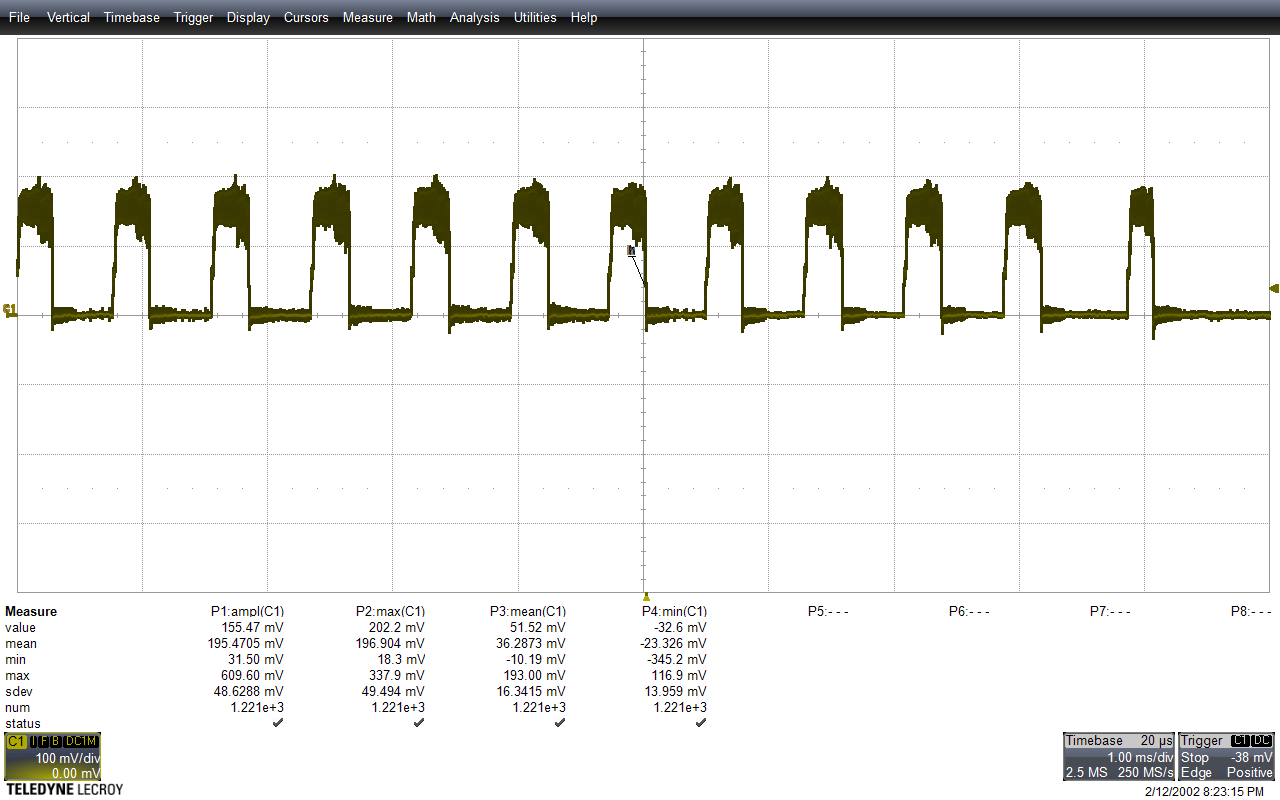
\includegraphics[width=0.47\textwidth]{Mediciones/P02_reposo_sin_cap_entrada.png}}
  \subfigure[Con capacitores de entrada]{
    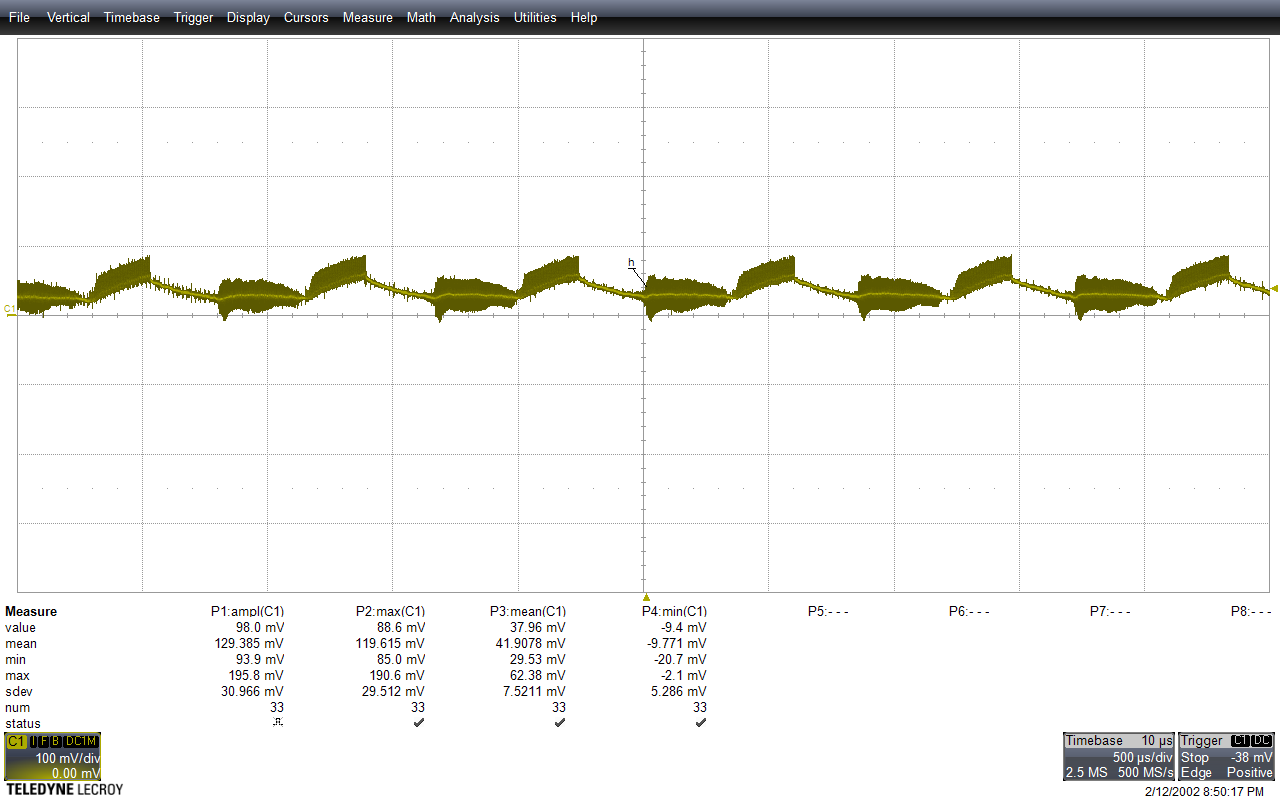
\includegraphics[width=0.47\textwidth]{Mediciones/P02_reposo_con_cap_entrada.png}}
 \caption{Corriente de entrada a \SI{12}{\volt} con la mano en reposo (canal invertido, \SI{100}{\milli\volt}/div $\equiv$ \SI{0.2}{\ampere}/div; base de tiempo de \SI{1}{\milli\second}/div y \SI{500}{\micro\second}/div).}
 \label{fig:reposo_cap}
\end{figure}

\paragraph{Movimiento y servo bloqueado.} Al mover la muñeca en sus dos ejes a la vez (figura~\ref{fig:carga}a), la corriente media en la ventana de \SI{10}{\milli\second} de la captura es de unos \SI{0.21}{\ampere}, con picos de \SI{0.6}{\ampere}; el máximo registrado entre todas las adquisiciones fue de unos \SI{0.72}{\ampere}. Al bloquear a mano un servo (figura~\ref{fig:carga}b), la corriente se mantiene en unos \SIrange{0.55}{0.6}{\ampere} y el regulador conmuta en forma continua. El corte de la corriente de unos \SI{0.4}{\milli\second} al final de esa captura corresponde al instante en que se soltó el servo: deja de exigir corriente y el regulador deja de conmutar por un momento, hasta volver al régimen de reposo. No es una falla.

\begin{figure}[H]
 \centering
  \subfigure[\textit{Pitch} y \textit{roll} simultáneos (canal invertido, \SI{100}{\milli\volt}/div $\equiv$ \SI{0.2}{\ampere}/div)]{
    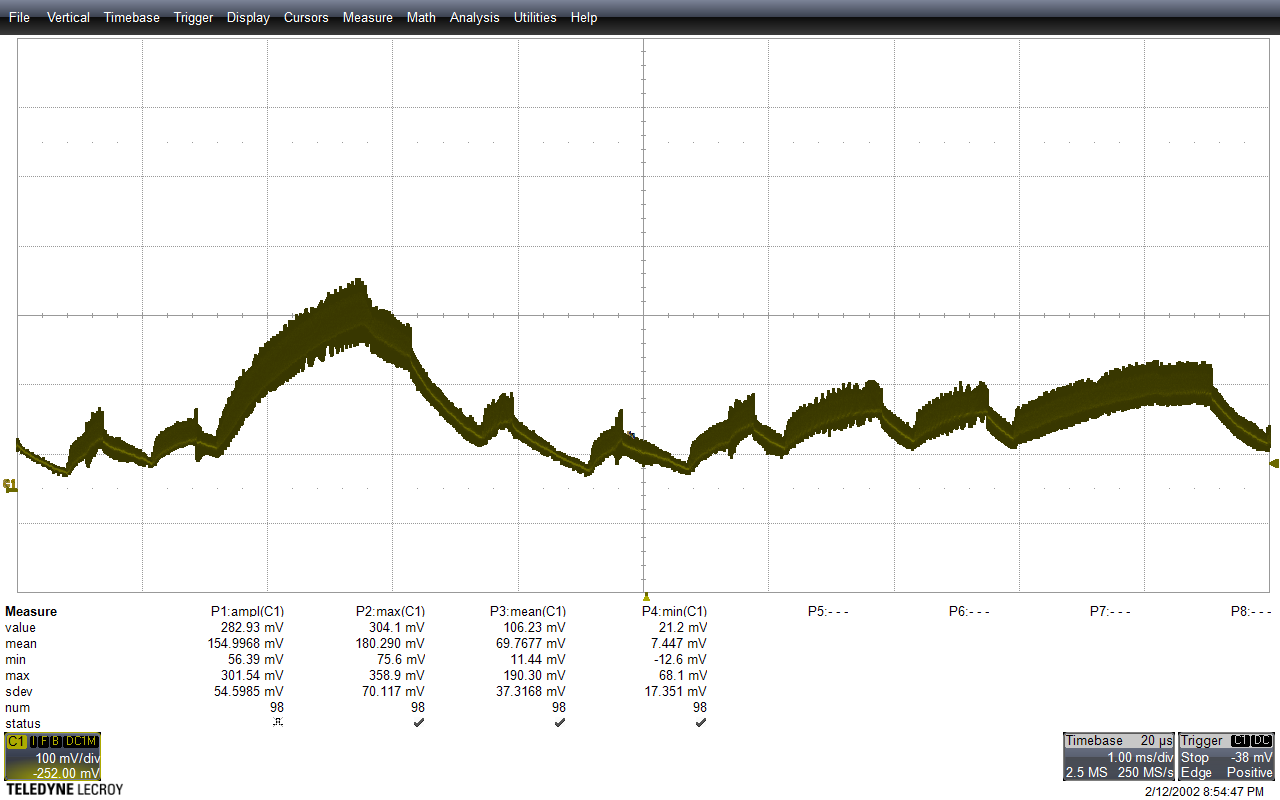
\includegraphics[width=0.47\textwidth]{Mediciones/P03_pitch_roll_con_cap.png}}
  \subfigure[Servo bloqueado (\SI{200}{\milli\volt}/div $\equiv$ \SI{0.4}{\ampere}/div)]{
    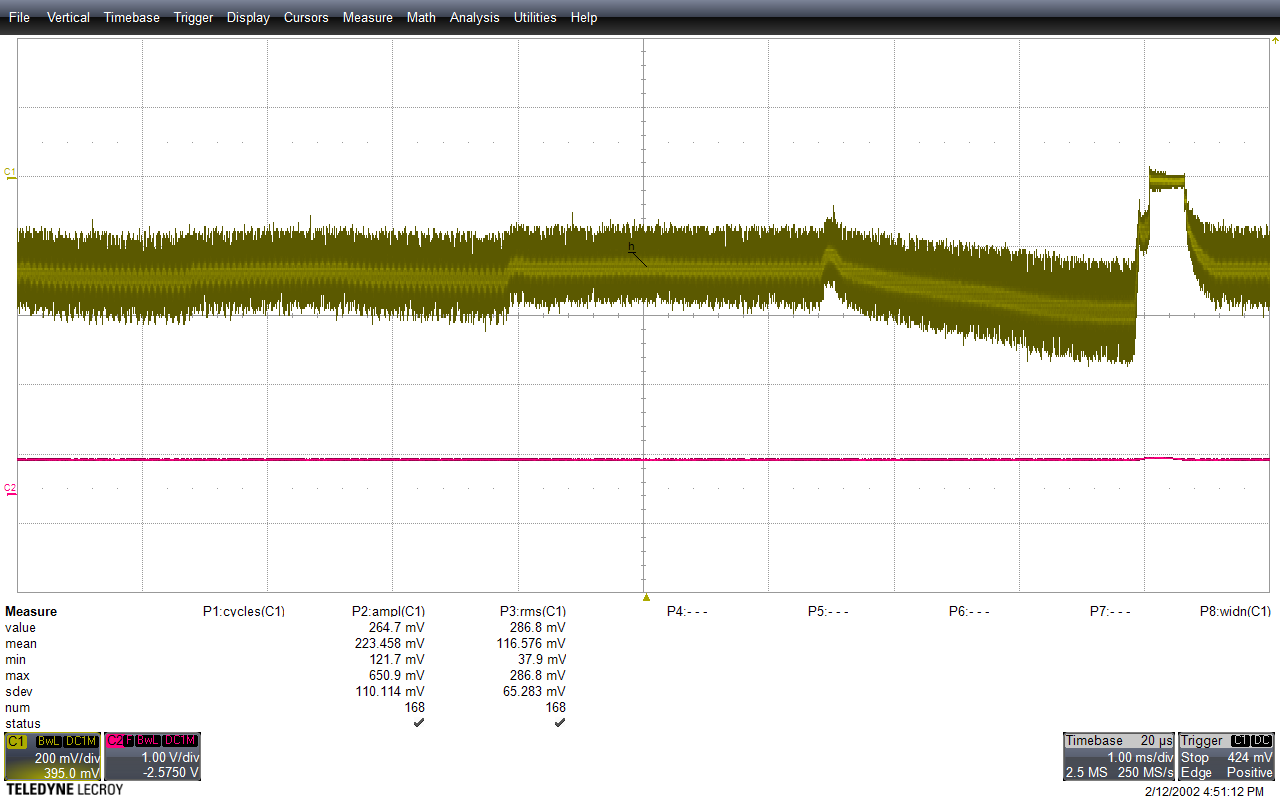
\includegraphics[width=0.47\textwidth]{Mediciones/P03_servo_bloqueado.png}}
 \caption{Corriente de entrada a \SI{12}{\volt} con carga (\SI{1}{\milli\second}/div).}
 \label{fig:carga}
\end{figure}

\paragraph{Tensión de salida.} El valor eficaz de la línea de \SI{5}{\volt} de los servos se mantuvo entre \SI{5.14}{\volt} y \SI{5.25}{\volt} en 57 adquisiciones, con un desvío de \SI{16}{\milli\volt} (figura~\ref{fig:v5}). En la traza se ven ondulaciones breves de algunas décimas de volt; con la escala de \SI{1}{\volt}/div utilizada no es posible resolver el rizado con más detalle, y el parámetro de amplitud del osciloscopio no es confiable en esas condiciones, por lo que se toma como referencia el valor eficaz.

\begin{figure}[H]
    \centering
    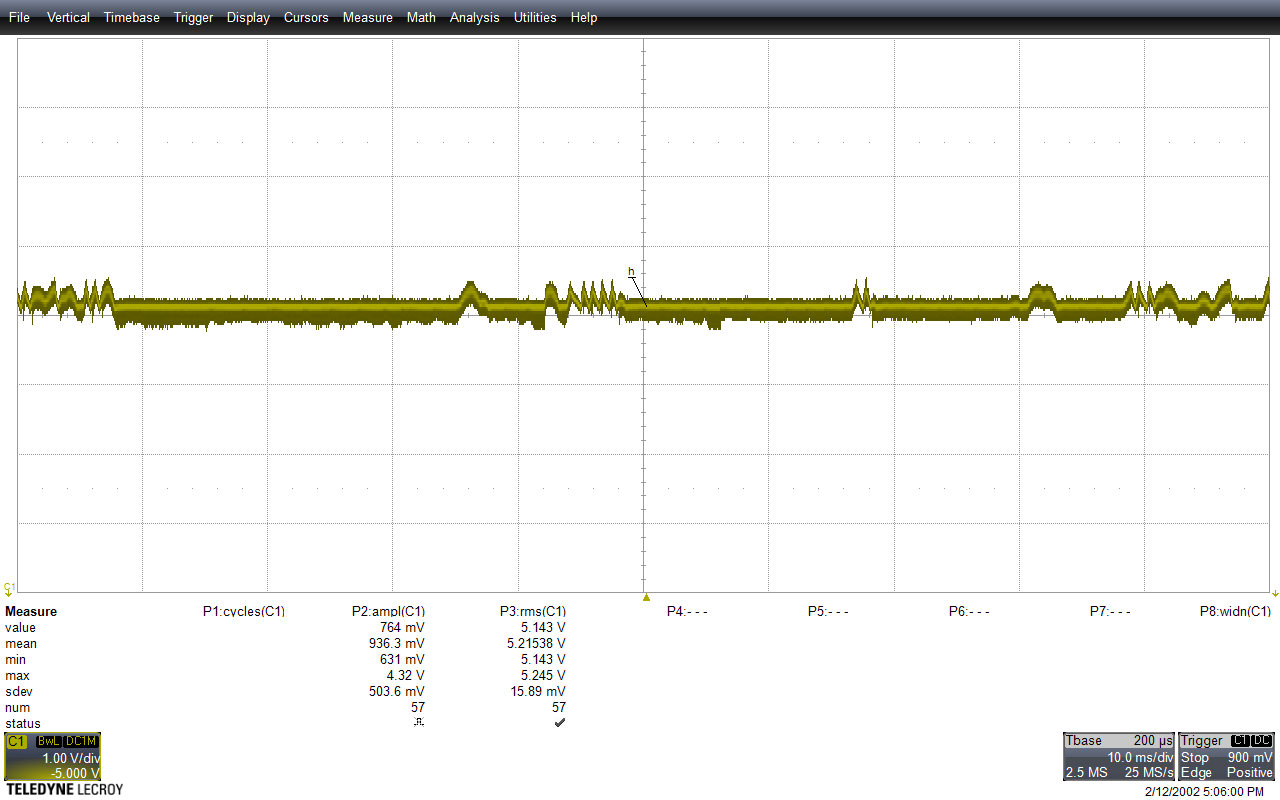
\includegraphics[width=0.7\textwidth]{Mediciones/P02_V5_regulador.png}
    \caption{Tensión de salida del regulador (\SI{1}{\volt}/div, \SI{10}{\milli\second}/div, límite de ancho de banda activado).}
    \label{fig:v5}
\end{figure}

\paragraph{Conclusiones de las mediciones.} El consumo del receptor queda muy por debajo de la capacidad de la fuente (\SI{4}{\ampere}) y del regulador (\SI{3}{\ampere} a la salida): aun en el peor caso registrado, la corriente de entrada no superó los \SI{0.75}{\ampere} a \SI{12}{\volt}. Los picos de bloqueo de los MG946R estimados en la sección~\ref{sec:alimentacion} con las hojas de datos no se presentaron en el uso normal, lo que es coherente con la acción del limitador de velocidad, aunque no se midió el consumo sin él. La línea de \SI{5}{\volt} también se observó con la mano en movimiento y su valor casi no varió, por lo que los picos de corriente no comprometen la alimentación de los servos. No se midió la corriente media en movimiento continuo durante un tiempo prolongado.
